\documentclass[
12pt,
openany, %openright,			
oneside, %twoside,			%% twoside: para frente e verso ao imprimir
a4paper,			
english,			
%	french,				%% Idioma adicional 
%	spanish,			%% Idioma adicional 
brazil			        %% Idioma principal 
]{abntbibufjf}

\usepackage{lmodern}						
\usepackage[T1]{fontenc}		
\usepackage[utf8]{inputenc}		%% Para converter automaticamente acentos como digitados. Mude utf8 para latin1 se precisar. 
%% Permite digitar os acentos no teclado normalmente, sem comandos (\'e \`a , etc.).
\usepackage{lastpage}			
\usepackage{indentfirst}		
\usepackage{color}			
\usepackage{graphicx}			
\usepackage{microtype} 
\usepackage{verbatim}
\usepackage{array}	
\usepackage{amsfonts}
\usepackage{amsmath}
\usepackage{amssymb}
\usepackage{amstext}
\usepackage{amsthm}
\usepackage[alf]{abntex2cite}
%\usepackage{subcaption}
\usepackage{multirow}
\usepackage{pythontex}

\usepackage{blindtext}

\newcommand{\verm}{\textcolor[rgb]{1.00,0.00,0.00}}
\newcommand{\green}{\textcolor[rgb]{0.00,0.70,0.00}}
\newcommand{\blue}{\textcolor[rgb]{0.00,0.00,1.00}}
\newcommand{\purp}{\textcolor[rgb]{0.52,0.00,0.90}}

\newcommand{\exu}[1]{\textcolor{red}{#1}}

\usepackage{listings}
\definecolor{mygreen}{RGB}{28,172,0} % color values Red, Green, Blue
\definecolor{mylilas}{RGB}{170,55,241}

\usepackage{hyperref}
\hypersetup{
    colorlinks=true,
    linkcolor=black,
    urlcolor=black,
    citecolor = black,
}

\urlstyle{same}

\lstset{language=Matlab,%
    %basicstyle=\color{red},
    breaklines=true,%
    morekeywords={matlab2tikz},
    keywordstyle=\color{blue},%
    morekeywords=[2]{1}, keywordstyle=[2]{\color{black}},
    identifierstyle=\color{black},%
    stringstyle=\color{mylilas},
    commentstyle=\color{mygreen},%
    showstringspaces=false,%without this there will be a symbol in the places where there is a space
    numbers=left,%
    numberstyle={\tiny \color{black}},% size of the numbers
    numbersep=9pt, % this defines how far the numbers are from the text
    emph=[1]{for,end,break},emphstyle=[1]\color{blue}, %some words to emphasise
    emph=[2]{all}, emphstyle=[2]\color{mylilas},    
}

%\usepackage[square,sort,comma,numbers]{natbib}

\def\dohyo{\textit{dohy}$\bar{o}$} % dohyo
\def\lego{LEGO\raisebox{5pt}{\tiny\textregistered}} % LEGO
\def\matlab{MATLAB\raisebox{5pt}{\tiny\textregistered}} % MATLAB

\DeclareMathOperator{\sen}{sen}

%% -----------------------------------------------------------------------------

%% Obs.: Alguns acentos foram omitidos.

\titulo{Automação Residencial utilizando IoT} %%Por exemplo, Titulo da tese
% \subtitulo{: subt\'itulo do trabalho}  %% Retirar o primeiro ``%'' desta linha se for utilizar subtitulo. Deixar os dois pontos antes, em ``: subt\'itulo'' . 
\autor{Rayssa Soares de Oliveira}
%\autorR{Sobrenome, Nome} %%Colocar o sobrenome do autor antes do primeiro nome do autor, separados por ,
\local{Juiz de Fora}
\data{2021} %%Alterar o ano se precisar
\orientador[Orientador:]{Exuperry Barros Costa} %%Se precisar, troque [Orientador:] por [Orientadora:]
%\coorientador[Coorientadora:]{NOME AQUI} %% Retirar o primeiro ``%'' desta linha se tiver coorientador. Se precisar, troque por [Cooorientadora:]. 
\instituicao{UNIVERSIDADE FEDERAL DE JUIZ DE FORA}
\faculdade{DEPARTAMENTO DE ENERGIA} %%Alterar, dentro de chaves {}, se precisar.
\programa{ENGENHARIA ELÉTRICA - HABILITAÇÃO EM ROBÓTICA E AUTOMAÇÃO INDUSTRIAL} %%Alterar, dentro de chaves {}, se precisar.
\objeto{Disserta\c{c}\~ao}  %%Tese (Doutorado)
\natureza{Trabalho de Conclusão de Curso
apresentado
	à Faculdade de Engenharia da Universidade
	Federal de Juiz de Fora, como requisito parcial
	para a obtenção do título de Bacharel em
	Engenharia Elétrica.} %%Trocar Matem\'atica por outro, se precisar.


%% Abaixo, preencher com os dados da parte final da ficha catalografica

%\finalcatalog{1. Análise computacional de tensões de imagens obtidas por fotoelasticidade. 2. Escala de tensões baseada em cores das franjas fotoelásticas. 3. Fotoelasticidade digital. I. Scari, Alexandre da Silva, orient. II. T\'itulo.} %% Aqui fica 
% escrito a palavra ``T\'itulo'' mesmo, nao o do trabalho. Se tiver coorientador, os dados ficam depois dos dados 
%% do orientador (II. Sobrenome, Nome do coorientador, coorient.) e antes de ``II. T\'itulo'', o qual passa a ``III. T\'itulo''.

%% ---

\setlength{\parindent}{1.3cm}

\setlength{\parskip}{0.2cm}  

\setlength\afterchapskip{12pt}  

%% Iniciar o documento
\begin{document}
	
	%% ELEMENTOS PRE-TEXTUAIS
	
	%% Capa
	\inserecapa
	
	%% Folha de rosto
	\inserefolhaderosto
	
	
	%% Ficha catalografica. AO IMPRIMIR, DEIXAR NO VERSO DA FOLHA DE ROSTO.
	%\inserecatalog  

	
	
	%% Folha de aprovacao

	\begin{folhadeaprovacao}
		
		\begin{center}
			{\chapterfont \bfseries \insereautor}
			
			\vfill
			\begin{center}
				{\chapterfont\bfseries\inseretitulo \inseresubtitulo}
			\end{center}
			\vfill
			
			\hspace{.45\textwidth}
			\begin{minipage}{.5\textwidth}
				\inserenatureza
			\end{minipage}%
			\vfill
		\end{center}
		
		Aprovado em 26 de Março de 2021. 
		
		\begin{center} BANCA EXAMINADORA \end{center}
		\assinatura{Professor Dr. \insereorientador \ - Orientador \\ Universidade Federal de Juiz de Fora} 
		%\assinatura{Professora Dra. \inserecoorientador \ - Coorientadora \\ Universidade Federal de Juiz de Fora}
		\assinatura{Prof. Leonardo Rocha Olivi - Avaliador \\ Universidade Federal de Juiz de Fora}
		%\assinatura{}
		%  \assinatura{...} %%RETIRE O % E PREENCHA SE PRECISAR
		%  \assinatura{...}
		%  \assinatura{...}
	\end{folhadeaprovacao}
	
	
	%% Dedicatoria. OPCIONAL. Retirar o ``%'' de cada das 4 linhas abaixo, caso queira.
	% \begin{dedicatoria} \vspace*{\fill} \centering \noindent
	%   \textit{ Dedico este trabalho ... (opcional)} 
	%   \vspace*{\fill}
	% \end{dedicatoria}
	
	
	%% Agradecimentos. OPCIONAL. CASO SEJA BOLSISTA, INSERIR OS DEVIDOS AGRADECIMENTOS.
	\begin{agradecimentos}
		
		
	Agradeço à minha família pelo apoio e suporte em todos os momentos da vida. Sempre se fizeram presentes, me incentivando a nunca desistir dos meus objetivos e sendo meu alicerce ao longo de toda minha trajetória. Me ensinaram que sempre devemos aproveitar as oportunidades que a vida nos dá e, graças a eles, concluo a mais uma etapa da minha vida.
	
	Aos meus amigos, sou grata pela amizade e apoio de sempre. Sua presença ao longo da graduação foi essencial para que os obstáculos não parecessem tão difíceis. Juntos pudemos trocar momentos de alegria e tristeza que foram parte importante desses últimos anos.
	
	Ao meu querido companheiro, Filipe, sou grata pelo apoio, carinho, atenção e companheirismo que foram peças chaves para nosso relacionamento. Em momentos difíceis, seu apoio foi essencial para que eu prosseguisse na minha caminhada.
	
	À Faculdade de Engenharia da Universidade Federal de Juiz de Fora (UFJF) sou grata pelo acolhimento e ensino de qualidade. Dentro de um ambiente diversificado, tive contato com diferentes perspectivas e realidades. A UFJF foi espaço de valiosas transformações pessoais e profissionais.
	
	Aos meus professores, agradeço a dedicação, a atenção, a empatia, a paciência e todo conhecimento transmitido dentro e fora de sala de aula. Seu trabalho é admirável e de extrema importância para meu crescimento e minha formação.
	
	Aos meus orientadores, agradeço por todo \textit{feedback} recebido que foram cruciais para que eu me desenvolvesse e melhorasse a cada dia. Além de todo aprendizado, me ajudaram a me transformar na profissional que sou hoje, sempre agindo com ética e responsabilidade.
	
	Agradeço à equipe de competição de robótica da UFJF, a Rinobot, por todo aprendizado como desenvolvedora e capitã e pelas amizades que foram fundamentais para meu desenvolvimento. A minha trajetória na equipe foi o auge da minha graduação. Vivenciar essa atmosfera de competição foi um privilégio e me orgulho de ter feito parte desse time.
	
	Por fim, sou grata à todos que participaram direta ou indiretamente da minha trajetória.
	
	

		
	\end{agradecimentos}
	
	%% Epigrafe. OPCIONAL
	\begin{epigrafe}
		\vspace*{\fill}
		\begin{flushright}
			``Você se torna o que você acredita.''\\
			Oprah Winfrey.
		\end{flushright}
	\end{epigrafe}

	
	%% RESUMOS
	
	%% Resumo em Portugu^es. OBRIGATORIO.
	\setlength{\absparsep}{18pt} 
	\begin{resumo}
	
	    Domótica é a área do conhecimento e também da engenharia voltada ao desenvolvimento de soluções de automação residencial para dispor, aos seus usuários, maior conforto e segurança. Outra aplicação, que possui forte apelo social, é prover a acessibilidade a atividades e equipamentos aos portadores de necessidades especiais que, anteriormente, dependeriam da intervenção de outras pessoas. As soluções de automação residencial normalmente são compostas por um \textit{hardware} de controle, responsável pelo monitoramento de sensores e acionamento de dispositivos e um \textit{software} de gerenciamento do sistema, que dispõe de funcionalidades básicas de cadastramento de dispositivos, monitoramento de eventos e execução de comandos. Este trabalho  propõe o desenvolvimento um protótipo de um sistema de domótica de baixo custo composto por um \textit{hardware} de controle que se comunica com um \textit{smartphone} através de protocolo TCP/IP e um aplicativo para \textit{android} de gerenciamento, com acesso através da Internet. Este trabalho também tem o objetivo secundário demonstrar à viabilidade de soluções de baixo custo, democratizando o acesso a automação residencial.
		
		
		Palavras-chave: Automação Residencial; Domótica; Internet das Coisas; MQTT; Iluminação Residencial.
		
	\end{resumo}
	
	
	%% Resumo em Inglês
	\begin{resumo}[ABSTRACT]
		\begin{otherlanguage*}{english}
			
			Home automation is the area of knowledge and also of engineering aimed at the development of home automation solutions to provide its users with greater comfort and safety. Another application, which has a strong social appeal, is to provide accessibility to activities and equipment for people with special needs that, previously, would have depended on the intervention of other people. Home automation solutions are usually composed of control hardware, responsible for monitoring sensors and triggering devices and system management software, which has basic functionality for registering devices, monitoring events and executing commands. This work proposes the developmet of a prototype of a low-cost home automation system composed of control hardware that communicates with a smartphone through the TCP / IP protocol and an application for management android, with access through the Internet. This work also has the secondary goal of demonstrating the viability of low-cost solutions, democratizing access to home automation. 
			
			

			
			Keywords: Home Automation; Domotics; Internet of Things; MQTT; Residential Lighting.
		\end{otherlanguage*}
	\end{resumo}

	
	%% Seguindo o mesmo modelo acima, pode-se inserir resumos em outras linguas. 
	
	%% Lista de ilustracoes. OPCIONAL.
	\pdfbookmark[0]{\listfigurename}{lof}
	\listoffigures*
	\cleardoublepage
	
	
	%% Lista de tabelas. OPCIONAL.
	%\pdfbookmark[0]{\listtablename}{lot}
	%\listoftables*
	\cleardoublepage
	
	%% Lista de abreviaturas e siglas. OPCIONAL
	\begin{siglas}
	
	\item [ARP] \textit{Address Resolution Protocol}
	\item [ASHRAE3] \textit{American Society of Heating, Refrigerating and Air Conditioning Engineers}
	\item[AURESIDE] Associação Brasileira de Automação Residencial
	\item [CFTV] Circuito Fechado de Televisão
	\item [DNS] \textit{Domain Name System}
	\item [FTP] \textit{File Transfer Protocol}
	\item [GPIO] \textit{General Purpose Input/Output}
    \item [HTTP] \textit{Hypertext Transfer Protocol}
	\item [HVAC] \textit{Heating, Ventilation and Air Conditioning}
	\item [IBM] \textit{International Business Machines Corporation}
	\item [IoT] \textit{Internet of Things} - Internet das Coisas
	\item [IP] \textit{Internet Protocol}
	\item [IPX/SPX] (\textit{Internetwork Packet Exchange/Sequenced Packet Exchange})
	\item [LED] \textit{Light Emitting Diode}
	\item [MQTT] \textit{Message Queue Telemetry Transport}
	\item [NETBEUI] \textit{NetBIOS Extended User Interface}
	\item [OASIS] \textit{Organization for the Advancement of Structured Information Standards}
	\item [OSI] \textit{Open System Interconnection}
	\item [PC] \textit{Personal Computer}
	\item [RFB] \textit{Remote Frame Buffer protocol}
	\item [RFID] \textit{Radio-Frequency Identification}
	\item [SMS] \textit{Short Message Service}
	\item [SSH] \textit{Secure Socket Shell}
	\item [SSL] \textit{Secure Sockets Layer}
	\item [TCP] \textit{Transmission Control Protocol}
	\item [UART] \textit{Universal Asynchrounous Receiver/Transmiter}
	\item [UDP] \textit{User Datagram Protocol}
	\item [USB] \textit{Universal Serial Bus}
	\item [VNC] \textit{Virtual Network Computing}
	\item [XNS] \textit{Xerox Network System}
		
	\end{siglas}
	
	
	
	
	%% Lista de simbolos. OPCIONAL
	%\begin{simbolos}
	
	%\item [$net$] Ativação
	%\item [$\delta$] \textit{Bias}
 	
	%\end{simbolos}  
	
	
	
	
	%% Sumario
	\pdfbookmark[0]{\contentsname}{toc}
	\tableofcontents*
	\cleardoublepage
	
	%% ----------------------------------------------------------
	
	%% ELEMENTOS TEXTUAIS
	
	\textual
	\pagestyle{simple}   
	
	
	\chapter{INTRODUÇÃO} 
	\label{cap1}
	
	Automação é um “sistema automático pelo qual os mecanismos controlam seu próprio funcionamento, quase sem a interferência do homem” \cite{FERREIRA}. Em seu uso moderno, a automação pode ser definida como uma tecnologia que utiliza comandos programados para operar um dado processo, combinados com retroação de informação para determinar que os comandos sejam executados corretamente. Ela é frequentemente utilizada em processos, antes operados por seres humanos, é a aplicação de técnicas computadorizadas ou mecânicas para diminuir o uso de mão de obra em qualquer processo, especialmente o uso de robôs nas linhas de produção. A automação diminui os custos e aumenta a velocidade da produção.
	
	Também pode ser definida como um conjunto de técnicas que podem ser aplicadas sobre um processo a fim de torná-lo mais eficiente: maximizando a produção com menor consumo de energia, menor emissão de resíduos e melhores condições de segurança, tanto humana e material quanto das informações inerentes ao processo.
	
	A automação pode ser dividida em alguns ramos principais:

\begin{itemize}
    \item Automação industrial - Utilizada com máquinas ou processos. Consiste em escolher, entre as diversas tecnologias que se encontram ao nosso dispor, as que melhor se adaptam ao processo a desenvolver e a melhor maneira de as interligar para garantir sempre a melhor relação custo beneficio;
    \item Automação Residencial - Aplicação de técnicas para melhoria no conforto e segurança de residências e conjuntos habitacionais, tais como: Controle de acesso por biometria, porteiro e portões eletrônicos, CFTV (Circuito Fechado de Televisão), controle de luminosidade de ambientes, controle de HVAC (\textit{Heating, Ventilation and Air Conditioning}), etc.
\end{itemize}

    Para viabilizar a automação de um determinado processo, existe uma necessidade preliminar de realização de um estudo de engenharia básica ou levantamento de dados que verificará todas as necessidades para o processo. Serve como subsídio para a identificação, análise e determinação da melhor estratégia de controle e para a escolha dos recurso de hardware e/ou software necessários para a aplicação.

    Atualmente, a automação está presente em diferentes níveis de atividades do homem, desde residências, no trânsito, através de sistemas de controle de tráfego e sinalização, nos edifícios comerciais, processos de compra, venda e transporte de bens, processos industriais e até em jornadas espaciais.
    
    As expressões \textit{domótica}, \textit{casas inteligentes} e \textit{casas conectadas} também são usadas para se referir ao mesmo conceito. Domótica é a junção do latim \textit{domus}, que significa casa, com robótica, que se refere ao que é automatizado.
	
	\section{Indústria 4.0}

	O modelo que remete à quarta revolução industrial, conhecida como Indústria 4.0, teve início na Alemanha em meados de 2012, inicialmente, como um programa institucional – envolvendo empresas, universidades e governo – de atualização tecnológica, com o objetivo de aumentar a competitividade da indústria alemã e modernizar a já desenvolvida indústria local \cite{ALMEIDA}.
	
	Como consequência, o perfil da mão de obra mudou e os profissionais da Indústria 4.0 se tornaram cada vez mais polivalentes e desenvolveram conhecimentos interdisciplinares. À medida que esse movimento foi avançando, sistemas integrados de manufatura, que eram internamente integrados a sistemas da própria empresa, passaram a ser integrados em sistemas com armazenamento em nuvens de dados, em postos alocados no chão de fábrica, transmitindo informações sobre as condições de produção e comportamento dos sistemas das máquinas e integrando essas informações àquelas oriundas dos próprios clientes consumidores dos produtos \cite{ALMEIDA}.
	
	
	\begin{figure}[!htb]
		\centering
		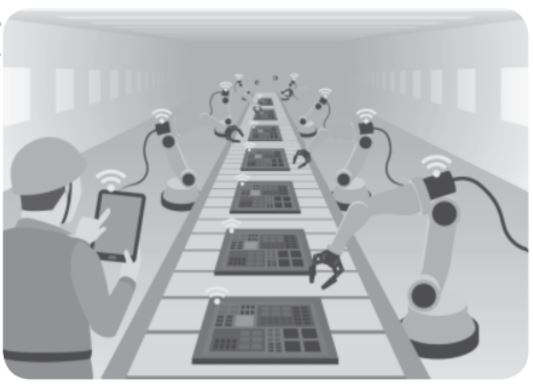
\includegraphics[scale=0.7]{Figuras/IoT.JPG}
		\caption{Sistema de produção com gerenciamento e produção de dados \textit{on-line}.}
		\label{VolatilidadePLD}
		\par Fonte: \cite{ALMEIDA}.
	\end{figure}
	
	
	A computação passou a ajudar pessoas a fazerem seus trabalhos de forma cada vez mais rápida e eficiente. Isso acarreta maior confiabilidade nas tarefas exercidas e também em um menor desgaste do usuário, que poderá realizar outras atividades mais complexas, implicando ganho de tempo e produtividade. 
	
	Nos últimos anos, além da atuação em ambientes industriais, a automação tem entrado no ambiente domiciliar, buscando maior comodidade e mais tempo de descanso para o usuário. Tendo isso em vista, foi desenvolvida uma nova área da automação, a domótica, que será abordada no Capítulo \ref{cap2}.
	
	
% 	\section{Trabalhos Relacionados}
% 	% ESCREVER ARTIGOS LIDOS QUE ESTÃO SENDO INSERIDOS NAS REFERÊNCIAS
% 	%% ESCREVER SOBRE OS ARTIGOS ...
	
% 	\citeauthor{Tonidandel} \exu{mexer aqui, parece que faltou alguma coisa}
	
%     \citeauthor{FAKIH}, por outro lado, compara as vantagens de se usar o próprio hardware para simulação de experimentos, considerando principalmente os custos da placa e dos componentes - REESCREVER 

%% Vamos deixar o Léo reclamar disso, e depois vc conserta, ok?
	
	
	
	\section{Objetivo}
	
	Tendo em mente os contratempos relacionados, assim como as melhorias citadas que podem ser adquiridas nos resultados, o objetivo deste trabalho é criar um sistema que automatiza a execução de determinadas tarefas residenciais remotamente, nesse caso o acionamento de uma lâmpada através de um aplicativo para \textit{smartphone}. Portanto, é fundamental nesse projeto a boa utilização das tecnologias acessíveis no mercado e conceitos de IoT (\textit{Internet of Things} - Internet das Coisas) importantes para automação residencial.
	
	De forma secundária, esse trabalho também objetiva demonstrar como evolução tecnológica pode auxiliar as pessoas em atividades cotidianas até mesmo doméstica, nesse caso.
	
	% falar sobre a utilização de coisas de baixo custo como um 2o parágrafo? Perguntar Exu
	
	%Resposta: sim! Seria bom. Se for o caso deixa pro pós correção do Léo



	\chapter{FUNDAMENTAÇÃO TEÓRICA}
	\label{cap2}
	\section{Internet das Coisas}
    
    A Internet das Coisas consiste na conexão entre rede de objetos físicos, ambientes, veículos e máquinas por meio de dispositivos eletrônicos, permitindo coleta e troca de informações. Na indústria de produtos e serviços, IoT representa diversas tecnologias que anteriormente não estavam ligadas e que, agora, estão conectadas por meio de uma rede baseada em endereços IP (\textit{Internet Protocol}). Com a aplicação da IoT à Indústria 4.0, um maior número de dispositivos vem sendo conectados por padrões tecnológicos, permitindo que dispositivos de campo se comuniquem e interajam uns com os outros \cite{ALMEIDA}.

    A evolução do IoT deve causar o próximo grande impacto no dia a dia das pessoas. É por meio do avanço desta tecnologia que será possível deixar a casa inteligente, com objetos e eletrônicos cada vez mais práticos, funcionais e autossuficientes. Em razão disso, além dos \textit{smartphones} e computadores pessoais, outros dispositivos poderão identificar padrões, processar informações e executar tarefas com apenas um (ou nenhum) clique. Hoje já é possível encontrar equipamentos e soluções de automação residencial conectados e integrados à aplicativos.
    
    A tecnologia está convergindo para produtos no estilo \textit{do yourself} ou \textit{plug and play}, isto é, o próprio usuário pode instalar e em poucos minutos já está pronto para utilização. A ideia é precisar de pouca infraestrutura para usufruir dos benefícios de uma casa inteligente. Basta apenas ter uma casa preparada para o IoT, com uma excelente conexão à internet.
    
    A Internet das Coisas veio para facilitar a instalação, o uso e ser muito mais acessível (em termos de custos de infraestrutura) a todos os usuários. Além da praticidade e intuitividade de utilização dos dispositivos, há muitos outros atrativos da automatização, podendo-se destacar o conforto e a segurança. Pela conexão à internet e dotados de “inteligência”, os eletrônicos e eletrodomésticos estarão integrados e se comunicando entre si, para tornar nossa vida mais fácil.

    Entre outros recursos como assistente virtuais e eletrodomésticos inteligentes, podem ser destacados os seguintes itens:

\begin{itemize}
    \item Lâmpadas inteligentes;
    \item Controle de acesso;
    \item Sistemas de segurança.
\end{itemize}

    Outra vantagem é a economia. Podendo controlar diversos sistemas remotamente, o usuário só liga aquilo que precisa e na hora que quer. É possível comandar as luzes, o ar condicionado, o uso da máquina de lavar roupa, entre outros como:

\begin{itemize}
    \item RFID (\textit{Radio-Frequency Identification});

    \item Interoperabilidade, comunicação entre objeto através de protocolos (\textit{WiFi}, \textit{Bluetooth}, \textit{Z-Wave}, outros);

    \item Interconectividade, capacidade de operação conjunta através de centrais (\textit{hubs} ou \textit{gateways});

    \item Geração de dados a partir de sensores e atuadores, para transformação de energia em dados e transmiti-los;

    \item Capacidade de procedimento de dados local, evitando perdas de configurações e definições do usuário por meio de centrais ou nuvem (\textit{analytics cloud}).

\end{itemize}

    Para a construção de um projeto robusto de automação residencial - isto é, que integre todos os subsistemas (segurança, iluminação, ar-condicionado, etc.) - são utilizados dispositivos que explicitam esta capacidade de forma técnica (sensores, atuadores, módulos). Na camada digital, o processamento em nuvem é utilizado para a análise segura dos dados recolhidos em tempo real e o gerenciamento do status de cada equipamento da solução.
    
	
	\section{Pilha TCP/IP}
	
	Os protocolos de comunicação mais importantes eram o TCP/IP (\textit{Transmission Control Protocol/Internet Protocol}), NETBEUI( \textit{NetBIOS Extended User Interface}), IPX/SPX (\textit{Internetwork Packet Exchange/Sequenced Packet Exchange}), XNS (\textit{Xerox Network System}) e o \textit{Apple Talk}, antes da internet se tornar tão comum. Com o acesso crescente e a popularização da Internet e com a necessidade de redes internas de empresas se conectarem com mais frequência à Internet, o protocolo TCP/IP expandiu-se também a estas redes empresariais, tornando-se atualmente no protocolo padrão de comunicação.
	
	Para que dois equipamentos de rede possam se comunicar, é necessário que ambos entendam as mesmas regras, isto é, o protocolo de comunicação deve ser o mesmo. É um protocolo estruturado por camadas na qual cada camada utiliza e presta serviços às camadas adjacentes. Cada camada trata das informações que correspondem apenas à sua função. \cite{FEUP}
	
	Existem 4 camadas distintas que formam o TCP/IP. A Figura \ref{modeloTCP} apresenta um comparativo entre o modelo de referência OSI (\textit{Open System Interconnection}) e a pilha TCP/IP.
	
	
	
	\begin{itemize}
	    \item \textbf{Camada de Acesso à Rede} – Agrega funções da camada física e da camada de ligação de dados presentes no modelo OSI. Ela lida com o \textit{hardware} da interface de rede, com a estrutura dos \textit{frames}, com o endereçamento físico, com o controle de acesso à rede e com a utilização do meio físico para comunicação. Nela também é feito o encapsulamento dos pacotes IP em \textit{frames} e a tradução dos endereços lógicos da rede em endereços físicos;
	    \item \textbf{Camada Rede} – Posicionamento do IP. Responsável pela circulação dos pacotes com base no endereço de destino. Neste nível pode também ser realizada a fragmentação e a remontagem de pacotes;
	    \item \textbf{Camada de Transporte} – É responsável pela transferência de dados entre duas máquinas. Na camada de transporte destacam-se os protocolos UDP (\textit{User Datagram Protocol}) e TCP. O TCP é o protocolo mais usado porque fornece garantia na entrega dos pacotes. A conexão TCP entre as máquinas emissora e receptora é feita através do \textit{Three-way Handshake}. O UDP é um protocolo mais simples e por si só não fornece garantia na entrega dos pacotes;
	    \item \textbf{Camada de aplicação} – Os serviços que dão suporte a processos de aplicação são encontrados nesse nível. Alguns exemplos de protocolo de aplicação são: \textit{Telnet} (protocolo de terminal virtual), HTTP (\textit{Hypertext Transfer Protocol}), DNS (\textit{Domain Name System}) e FTP (\textit{File Transfer Protocol}) \cite{FEUP}.
	\end{itemize}

	\begin{figure}[!htb]
		\centering
		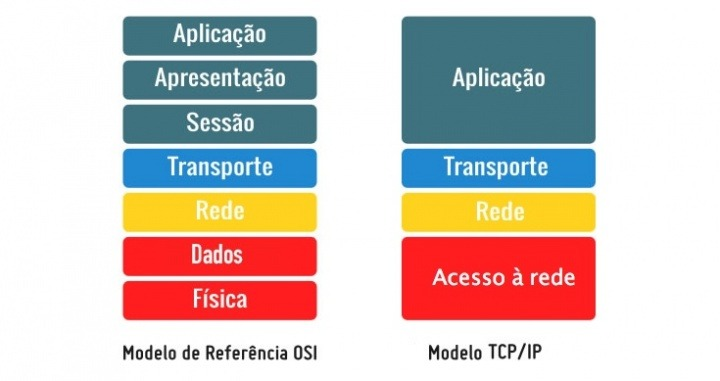
\includegraphics[scale=0.5]{Figuras/TCP-720x381.jpg}
		\caption{Modelo OSI \textit{versus} modelo TCP/IP}
		\label{modeloTCP}
		\par Fonte: \cite{PPLWARE}.
	\end{figure}

	
	\section{Protocolo MQTT}
	
	O MQTT (\textit{Message Queue Telemetry Transport}) foi inventado e desenvolvido inicialmente pela IBM (\textit{International Business Machines Corporation}) no final dos anos 90. Sua aplicação original era vincular sensores em \textit{pipelines} de petróleo a satélites. Ele é um protocolo de mensagem com suporte para a comunicação assíncrona. Um protocolo de sistema de mensagens assíncrono desacopla o emissor e o receptor da mensagem tanto no espaço quanto no tempo e, portanto, é escalável em ambientes de rede que não são confiáveis \cite{IBM}.
	
	Apesar do nome, o protocolo não tem relação com filas de mensagens, na verdade, ele usa um modelo de publicação e assinatura. No final de 2014, ele se tornou oficialmente um padrão aberto OASIS (\textit{Organization for the Advancement of Structured Information Standards}), com suporte nas linguagens de programação populares, usando diversas implementações de \textit{software} livre.
	
	O MQTT é um protocolo de rede leve e flexível que oferece o equilíbrio ideal para os desenvolvedores de IoT:

\begin{itemize}
    \item Permite a implementação em \textit{hardware} de dispositivos altamente restritos e em redes de largura da banda limitada e de alta latência;
    \item Sua flexibilidade possibilita o suporte a diversos cenários de aplicativo para dispositivos e serviços de IoT.
\end{itemize}


	Independente do setor econômico é possível encontrar um ambiente que precise ser controlado. Alguns desses ambientes precisam ser constantemente monitorados, visto que precisam operar em condições ideais.
	
	O monitoramento é a base da atividade de gerenciamento que consistem em acompanhar atividades importantes. No gerenciamento, os dados são constantemente coletados, oferecendo ao usuário as informações monitoradas. É possível criar uma base de conhecimento para que decisões possam ser tomadas corretamente, a partir dos indicadores apropriados.
	
	Alguns fatores de segurança de um \textit{Data Center}, por exemplo, que podem ser importantes para o monitoramento, são a temperatura e a umidade do ar \cite{ZUCCHI}. Segundo a ASHRAE3 (\textit{American Society of Heating, Refrigerating and Air Conditioning Engineers}), é ideal que a temperatura de \textit{Data Centers} esteja entre 18$^{\circ}$ C e 27$^{\circ}$ C e que a umidade relativa do ar esteja entre 40\% e 55\% \cite{ZEITTEC}. Para realizar esse controle, é possível desenvolver uma aplicação IoT utilizando o protocolo MQTT para realizar a comunicação entre os sensores que capturam a temperatura e a umidade do ar, o \textit{broker}, que concentra essas informações, e os objetos responsáveis pelas operações corretivas, caso os valores ideais não sejam alcançados.

    
	\begin{figure}[!htb]
		\centering
		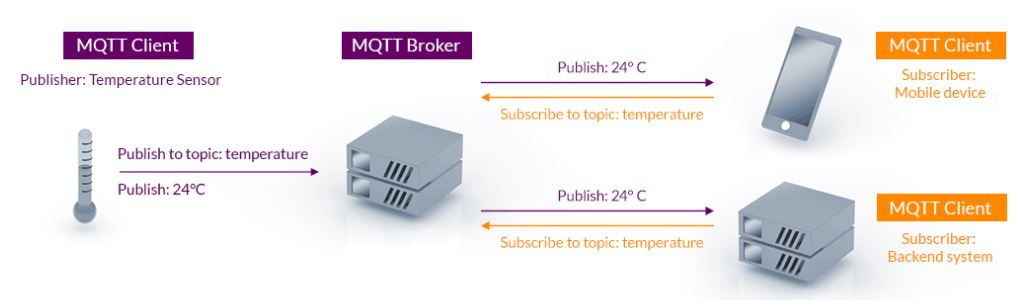
\includegraphics[scale=0.5]{Figuras/12.JPG}
		\caption{\textit{MQTT Publish}/Arquitetura de Publicação}
		\label{protocoloMQTT}
		\par Fonte: \cite{MQTT}.
	\end{figure}
	
    A Figura \ref{protocoloMQTT} ilustra o funcionamento da aplicação proposta e os papeis dos principais componentes para a realização dessa aplicação. Um sensor que mede a temperatura publica a informação no \textit{broker} através do protocolo MQTT. O \textit{broker}, por sua vez, publica essa informação em todos os clientes que subscreveram a temperatura de 24$^{\circ}$ C.
	
    
    \section{Domótica}
    
    Domótica é uma tecnologia recente que é responsável pela gestão de recursos habitacionais. O termo nasceu da fusão da palavra \textit{Domus}, que significa casa, com a palavra \textit{Robótica}, que está ligada ao ato de automatizar, isto é, realizar ações de forma automática. \cite{SISLITE}
    
    A automação residencial, ou Domótica, inicialmente é referenciada como novidade que as vezes causa curiosidade pelo seu grau tecnológico e pela alusão ao futurismo, ao mesmo tempo que pode ser compreendida como um símbolo de status e modernidade. Numa visão realista, a automação residencial proporciona o conforto e a conveniência que qualquer ser humano deseja. Ela está se tornando necessidade e um excelente fator de economia, tal qual foi a evolução da telefonia celular nos anos 90 - era possível estar em um lugar e falar no telefone com sua mãe em outro.
    
    Segundo José Cândido Forti, presidente da AURESIDE (Associação Brasileira de Automação Residencial), o objetivo da domótica é transformar casas em refúgios confortáveis que são capazes de economizar gastos e oferecer segurança. O que antes parecia ser um privilégio apenas da família \textit{Jetson} (seriado da TV dos anos 70), começa a se difundir nas residências de alto nível, transformando o conceito de casa do futuro em casa do presente. \cite{BUNEMER}
    
    Neste sentido, o assunto será tratado como uma realidade inevitável e que irá representar uma mudança incontestável nos atuais projetos de construção. Além do impacto nos profissionais e na forma de utilização do lar realmente como proporcionador de comodidade e satisfação.
    
    
    \section{Sistemas Embarcados}
    
    Atualmente, vários produtos possuem uma capacidade computacional eficaz e que estão presentes no dia a dia. Eletrodomésticos contam com sistemas eficazes para garantir maior conforto e praticidade aos usuários. No micro-ondas, é possível realizar diversas funções predefinidas pelo seu usuário. Neste equipamento um sistema embarcado está incluso.

    Um sistema embarcado consiste em um sistema microprocessado anexado ao produto e ao sistema que o controla. Ele é utilizado para realizar um conjunto de tarefas específicas e que foram previamente definidas. Com isso, é possível otimizar um determinado produto e diminuir o tamanho, bem como os recursos computacionais e o seu valor final. \cite{POZZEBOM}
    
    Um sistema embarcado pode ser definido como dispositivo que funcionam como computadores, que contam com memória, processador, interface de entrada e saída, porém, com o diferencial que desempenham uma tarefa específica, como o micro-ondas. Possuem aplicações no cotidiano e, por essa razão, às vezes não é possível mensurar sua capacidade computacional, já que estão tão envolvidos com tais mecanismos. Sistemas embarcados operam em máquinas que podem trabalhar por vários anos sem parar e, em alguns casos, possuem a capacidade de autocorreção.

    Um excelente exemplo de itens que usam sistemas embarcados são os \textit{smartphones} que desempenham funções específicas e que contam com mecanismos mais limitados que os computadores.

	\chapter{METODOLOGIA}
	\label{cap3}
	
	\section{\textit{Broker}}
	
    O \textit{broker} é um elemento fundamental na arquitetura \textit{publish-subscribers}. Dependendo da aplicação, pode ser necessário que esse elemento manipule milhões de mensagens simultâneas, com origem e destino em diversos clientes. O \textit{broker} é responsável por receber todas as mensagens, filtrá-las, determinar quem deve receber cada mensagem e enviar essas mensagens para os destinatários.
    
    Outra responsabilidade do \textit{broker} é autenticar e autorizar os clientes a enviar e/ou receber as mensagens. Assim, o \textit{broker} pode criar e manter sessões dos clientes autenticados, evitando que, a cada nova mensagem, a autenticação necessite ser realizada. Mensagens de conexão (início ou término) e de sessão são oferecidas pelo protocolo MQTT e foram apresentadas na Seção \ref{cap2}.
    
    O \textit{Eclipse Mosquitto4} é um exemplo de um \textit{broker}, implementado com código fonte aberto e que oferece suporte ao protocolo MQTT nas versões 3.1 e 3.1.1 \cite{OASIS}. Ele pode ser obtido gratuitamente e instalado nas mais diversas organizações. Adicionalmente, é possível encontrar diversos serviços na Internet que oferecem \textit{brokers online} que utilizam a implementação \textit{Eclipse Mosquitto}. Como exemplo, podem ser citados o \textit{Amazon IoT} (aws.amazona.com/iot), o \textit{Microsoft Azure} (azure.microsoft.com), o \textit{HiveMQ} (www.hivemq.com), o \textit{CloudMQTT} (cloudmqtt.com), entre outros.
    
    A utilização de um \textit{broker} na Internet (na nuvem), além de oferecer um serviço sem a necessidade da existência de um servidor dedicado a esse fim, permite que os clientes possam acessar esse serviço facilmente, a partir de qualquer ponto da Internet. A seguir é apresentado um desses \textit{brokers}, o CloudMQTT.
	
    
    \section{CloudMQTT}
    
    O CloudMQTT é uma implementação na nuvem do \textit{broker Mosquitto} que atualmente utiliza servidores da \textit{Amazon5} como suporte a essa aplicação. Depois do registro do usuário no sistema, é possível criar diversas instâncias, onde cada uma corresponde a um \textit{broker}. A Figura \ref{brokerMQTT} apresenta a tela de criação da instância \textit{TCC}, utilizada como exemplo neste trabalho. Nesse momento, além do nome da instância, é necessário escolher o plano de contratação. Para esta aplicação o plano \textit{Humble Hedgehog} é utilizado. Ele é o mais simples pago, uma vez que a opção gratuita não estava disponível, e atende os objetivos demonstrativos deste trabalho.
	
	O CloudMQTT tem suporte para linguagem \textit{Python}, que foi utilizada neste trabalho, mas ele também suporta outras plataformas como \textit{HTTP API}, \textit{Bridges}, \textit{Amazon Kinesis}, \textit{Heroku}, \textit{Ruby}, \textit{Node.js}, \textit{Java}, etc. Todos os tutoriais necessários para o aprendizado na linguagem \textit{Python} estão disponíveis na documentação do site da plataforma.
	
	\begin{figure}[!htb]
		\centering
		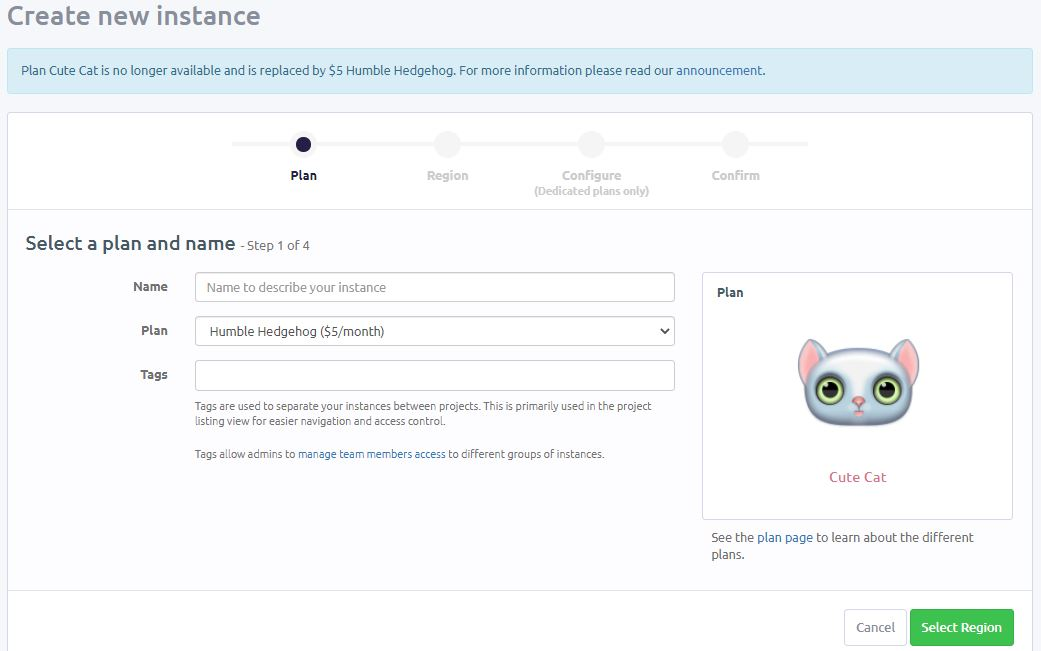
\includegraphics[scale=0.5]{Figuras/interfaceCriaInstancia.JPG}
		\caption{Criação do \textit{Broker on-line} no CloudMQTT}
		\label{brokerMQTT}
		\par Fonte: Autor, 2021.
	\end{figure}
	
	\begin{figure}[!htb]
		\centering
		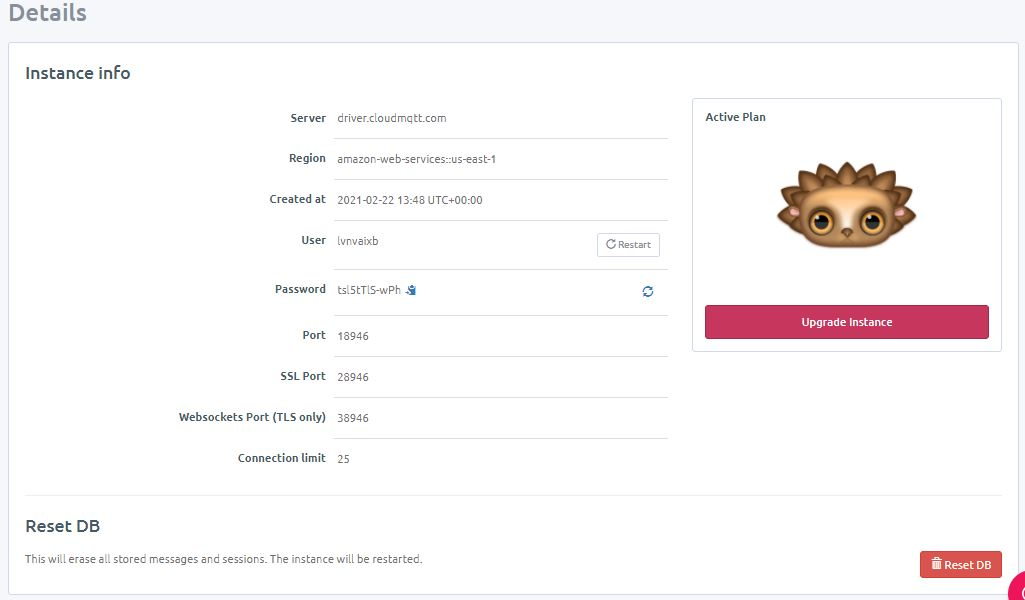
\includegraphics[scale=0.5]{Figuras/detalhesInstancia.JPG}
		\caption{Detalhes do \textit{Broker on-line} no CloudMQTT}
		\label{detalhesMQTT}
		\par Fonte: Autor, 2021.
	\end{figure}
	
	\section{MQTT \textit{Dash}}
	
	O MQTT Dash é um aplicativo \textit{mobile} para o sistema operacional \textit{Android} que pode ser utilizado para demonstração da comunicação em um cenário de IoT. Entre as suas funcionalidades, destacam-se a possibilidade de utilização de SSL (\textit{Secure Sockets Layer}) e de gráficos. Também é possível utilizar componentes como botões, áreas de texto e barras para envio de informações ao \textit{broker}. Na tela inicial do MQTT Dash é possível estabelecer a conexão ao \textit{broker} através do botão flutuante apresentado na Figura \ref{MQTTdash} à esquerda.
	
	
	\begin{figure}[!htb]
		\centering
		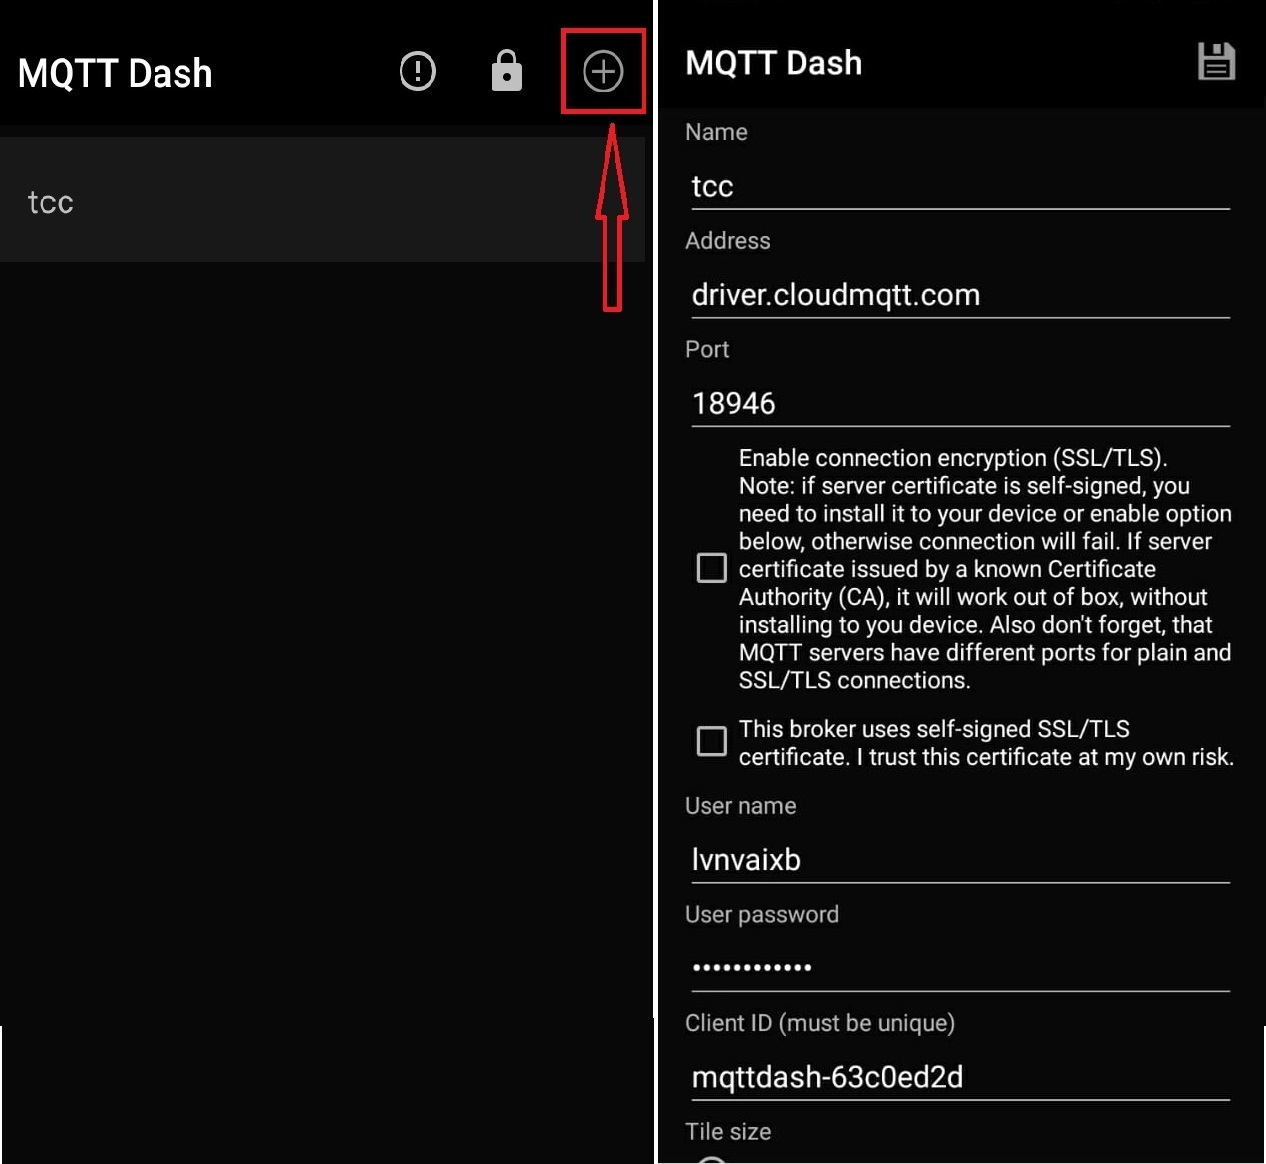
\includegraphics[scale=0.3]{Figuras/mqttDash.jpeg}
		\caption{Parâmetros do Cliente no aplicativo MQTT Dash}
		\label{MQTTdash}
		\par Fonte: Autor, 2021.
	\end{figure}
	
	
    \section{\textit{Raspberry Pi} 3}
    
    \begin{figure}[!htb]
		\centering
		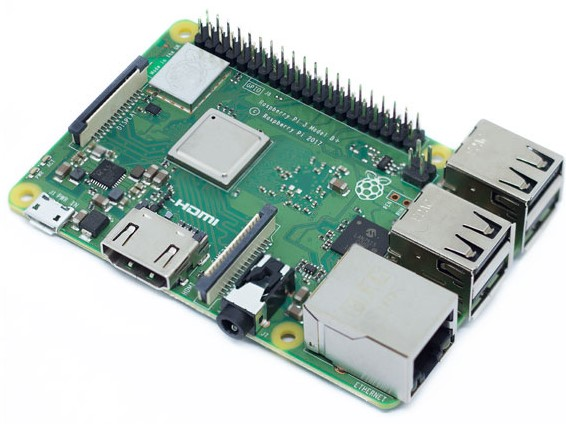
\includegraphics[scale=0.45]{Figuras/raspberry.jpeg}
		\caption{\textit{Raspberry Pi} 3}
		\label{raspberry}
		\par Fonte: \cite{FLOP}
	\end{figure}
    
    \textit{Raspberry Pi} é um computador de baixo custo e que tem o tamanho de um cartão de crédito desenvolvido no Reino Unido pela Fundação \textit{Raspberry Pi}. Seu sucesso deu-se pela facilidade na utilização e aplicação: conectar a um teclado e um mouse padrão a ele e conectar tudo isso a um monitor ou a uma televisão.
    
    O \textit{Raspberry Pi} 3 modelo B contem um processador 1.2GHz 64-bit quadcore ARMv8 CPU, 1 GB de RAM, \textit{Bluetooth} 4.1. A Figura \ref{GPIO} apresenta a pinagem da GPIO (\textit{General Pourpose Input/Output}) deste modelo. As GPIO são portas programáveis de entrada e saída de dados que são utilizadas para interface entre os periféricos e um microprocessador/microcontrolador.
    
    \begin{figure}[!htb]
		\centering
		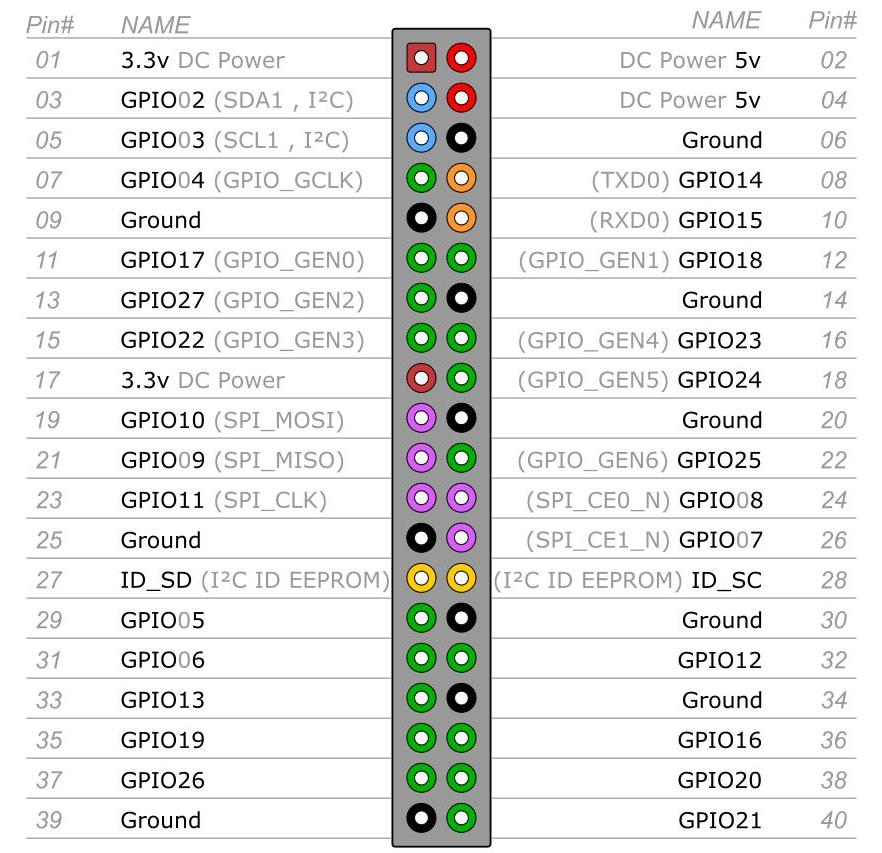
\includegraphics[scale=0.4]{Figuras/pi3_gpio.jpg}
		\caption{GPIO \textit{Header Raspberry Pi} 3}
		\label{GPIO}
		\par Fonte: \cite{ELEMENT}
	\end{figure}
	
	
	\subsection{Acesso ao \textit{Raspberry Pi}}
	
	O acesso ao \textit{Raspberry Pi} pode ser feito através de conexão SSH utilizando o \textit{software PuTTY SSH Client} cuja interface está representada na Figura \ref{putty}. Com o mesmo, é possível se conectar somente através do terminal do Ubuntu e as ações são feitas através de linha de comando, vide Figura \ref{Rasp-putty}.
	
	Caso o usuário opte por um acesso mais visual, é possível utilizar o VNC (\textit{Virtual Network Computing}),  um sistema de compartilhamento gráfico de \textit{desktop} que usa o RFB (\textit{Remote Frame Buffer protocol}) para controlar remotamente outro computador. Através deste protocolo o usuário pode conectar-se a um computador e utilizar as suas funcionalidades visuais como se estivesse sentado em frente dele.
	
	Uma das grandes vantagens é poder fazer a conexão de diferentes ambientes UNIX (Linux e outros) em Windows. VNC é independente da plataforma - há clientes e servidores para muitos \textit{GUI-based} sistemas operacionais e para Java. Múltiplos clientes se conectam ao \textit{VNC server} ao mesmo tempo. Geralmente essa tecnologia é usada para suporte técnico remoto e acesso de arquivos em um computador de trabalho de um computador de casa ou vice-versa.
	
	\begin{figure}[!htb]
		\centering
		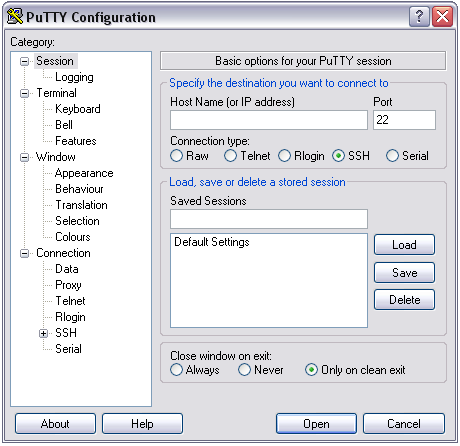
\includegraphics[scale=0.6]{Figuras/putty-portable.png}
		\caption{Interface \textit{PuTTY SSH Client}}
		\label{putty}
		\par Fonte: Autor, 2021.
	\end{figure}
	
	\begin{figure}[!htb]
		\centering
		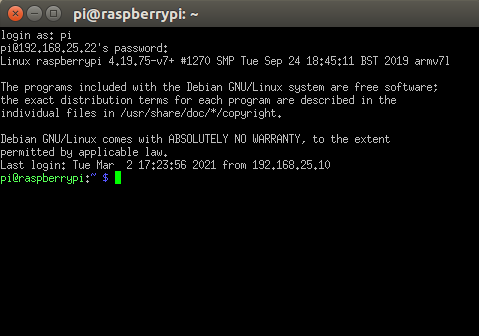
\includegraphics[scale=0.6]{Figuras/Raspberry-pelo-SSH.png}
		\caption{Raspberry acessado pelo \textit{PuTTY SSH Client}}
		\label{Rasp-putty}
		\par Fonte: Autor, 2021.
	\end{figure}
	
	O servidor do VNC é um programa instalado na máquina que compartilha sua tela. O servidor permite passivamente que o cliente tenha controle sobre ele. O protocolo VNC é muito simples, baseado em um gráfico primitivo do servidor para o cliente e envia mensagens do cliente para o servidor.
    
	\begin{figure}[!htb]
		\centering
		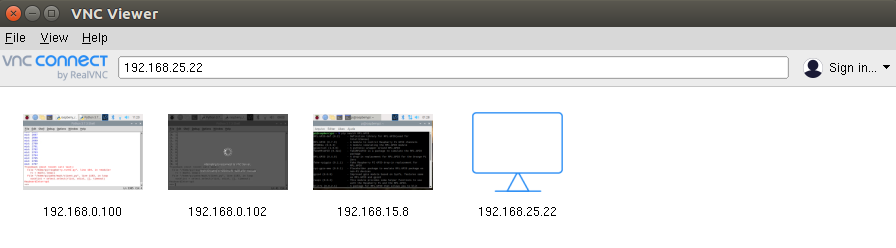
\includegraphics[scale=0.55]{Figuras/vnc2.png}
		\caption{Interface VNC}
		\label{vnc}
		\par Fonte: Autor, 2021.
	\end{figure}
	
    Para ambas as formas de acesso ao \textit{Raspberry} citadas no Capítulo \ref{cap3} é necessário, primeiramente, identificar o IP do \textit{Raspberry}. É possível obter tal informação através do terminal no Ubuntu através do comando \texttt{sudo ifconfig}. O endereço de IP do Raspberry aparece ao lado do IP do Wi-Fi conforme Figura \ref{terminalUbuntu}.
	
	\begin{figure}[!htb]
		\centering
		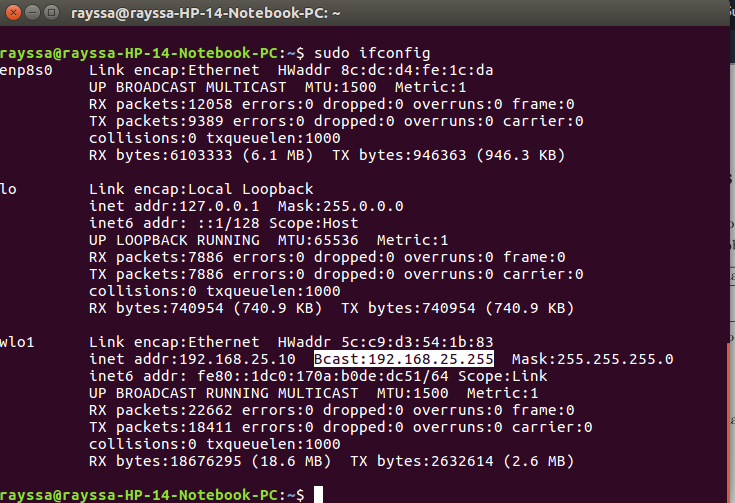
\includegraphics[scale=0.4]{Figuras/terminalUbuntu.png}
		\caption{Terminal Ubuntu}
		\label{terminalUbuntu}
		\par Fonte: Autor, 2021.
	\end{figure}
	
	\subsection{Raspbian}
	
	O sistema operacional instalado no \textit{Raspberry} é o \textit{Raspbian}. Ele é gratuito, baseado em \textit{Debian} e otimizado para o \textit{hardware Raspberry Pi}. Um sistema operacional é o conjunto de programas e utilitários básicos que fazem o \textit{Raspberry Pi} funcionar. No entanto, o \textit{Raspbian} oferece mais do que um sistema operacional puro: ele vem com mais de 35.000 pacotes, \textit{software} pré-compilado em um formato agradável para fácil instalação em seu \textit{Raspberry Pi}. \cite{RASPBIAN}

    \section{Projeto}
    
    Os materiais utilizados no projeto foram:
    
    \begin{itemize}
        \item \textit{Raspberry Pi Model B}
        \item Módulo relé para Arduino
        \item Lâmpada LED 127V/220V 9W
        \item Fio bitola $\phi$ 2,5mm
        \item Bocal para lâmpada de cerâmica
        \item \textit{Jumpers}
    \end{itemize}
    
    Apesar do comando de obtenção de IP citado acima ser comum em muitos tutoriais na Internet, ele não funciona em todos os casos. Neste caso, não foi possível identificar o IP através desse método.
	
	Foi utilizado o \textit{software Angry IP Scanner}, Figura \ref{angryIP}, como ferramenta para a obtenção do IP, $192.168.25.22$ do Raspberry para poder acessá-lo.
	
	\begin{figure}[!htb]
		\centering
		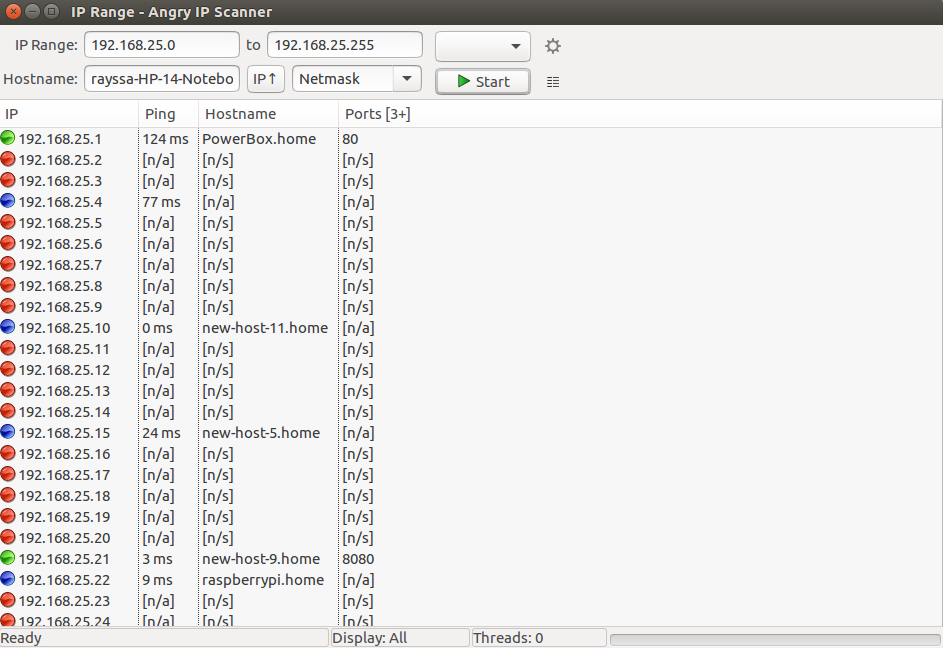
\includegraphics[scale=0.4]{Figuras/angryIP.png}
		\caption{Interface \textit{Angry IP Scanner}}
		\label{angryIP}
		\par Fonte: Autor, 2021.
	\end{figure}
	
    Foi elaborado um código em \textit{Python} para o sistema embarcado proposto. Nele está presente a lógica de comunicação juntamente com a lógica dos pinos de \textit{input} do \textit{Raspberry} para o acionamento dos relés.
    
    \begin{figure}[!htb]
		\centering
		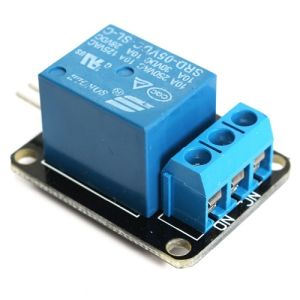
\includegraphics[scale=0.5]{Figuras/Modulo-rel-5V-DC-per-Arduino-e-Raspberry-Pi.jpg}
		\caption{Módulo relé Arduino 5V}
		\label{rele}
		\par Fonte: \cite{ROBOT}
	\end{figure}
    
    Na Figura \ref{montagem} encontra-se um esquemático da lâmpada que será acionada através do aplicativo no \textit{smartphone}. É possível notar que a lâmpada é ligada na rede 127V então a aplicação é feita de forma real podendo se utilizar em casa.
    
    \begin{figure}[!htb]
		\centering
		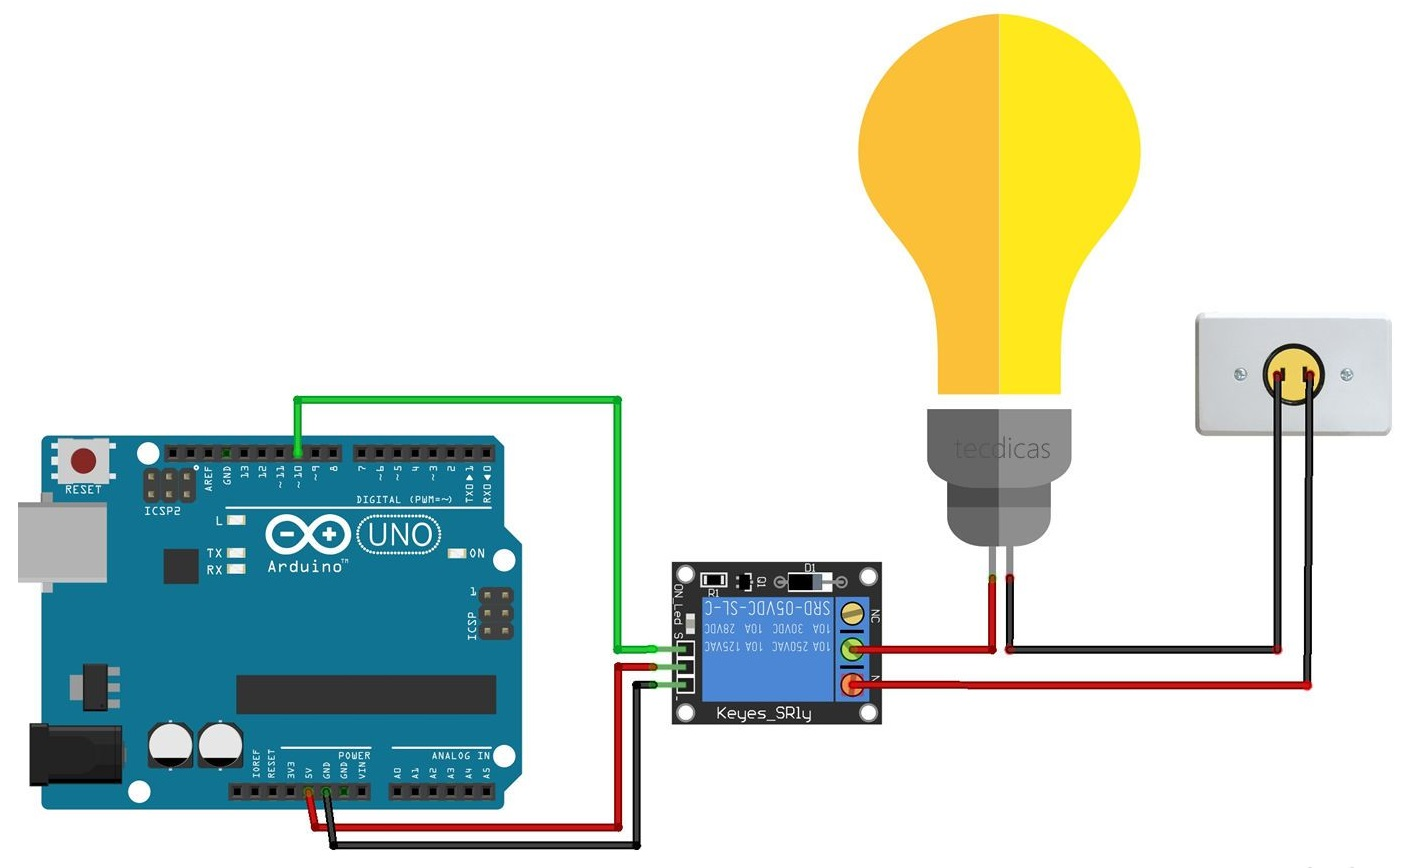
\includegraphics[scale=0.3]{Figuras/esquematico.jpg}
		\caption{Esquemático do \textit{hardware} do projeto}
		\label{montagem}
		\par Fonte: \cite{ELETRONICA}
	\end{figure}
    
    A Figura \ref{montagemFinal} ilustra o final do projeto: um acionamento de lâmpada através do Raspberry PI. Na imagem é representada uma placa de Arduino, mas no trabalho em questão foi utilizada uma placa de \textit{Raspberry Pi 3 Model B}.
    A GPIO 20 foi utilizada para o acionamento da lâmpada.
    
    
    
    \begin{figure}[!htb]
		\centering
		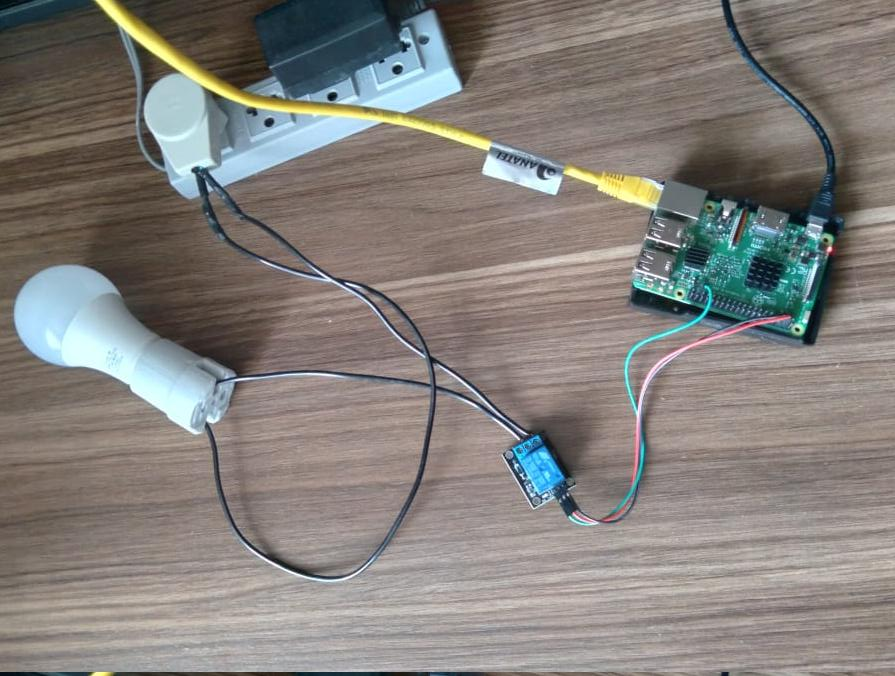
\includegraphics[scale=0.4]{Figuras/montagemFisica.jpeg}
		\caption{\textit{Hardware} do projeto}
		\label{montagemFinal}
		\par Fonte: Autor, 2021.
	\end{figure}
	
	O aplicativo, Figura \ref{app}, do projeto foi feito para acionar duas lâmpadas separadamente. Não foi possível a utilização de mais lâmpadas no \textit{hardware} devido a ausência de outro módulo relé ilustrado na Figura \ref{rele}. 
	
	\begin{figure}[!htb]
		\centering
		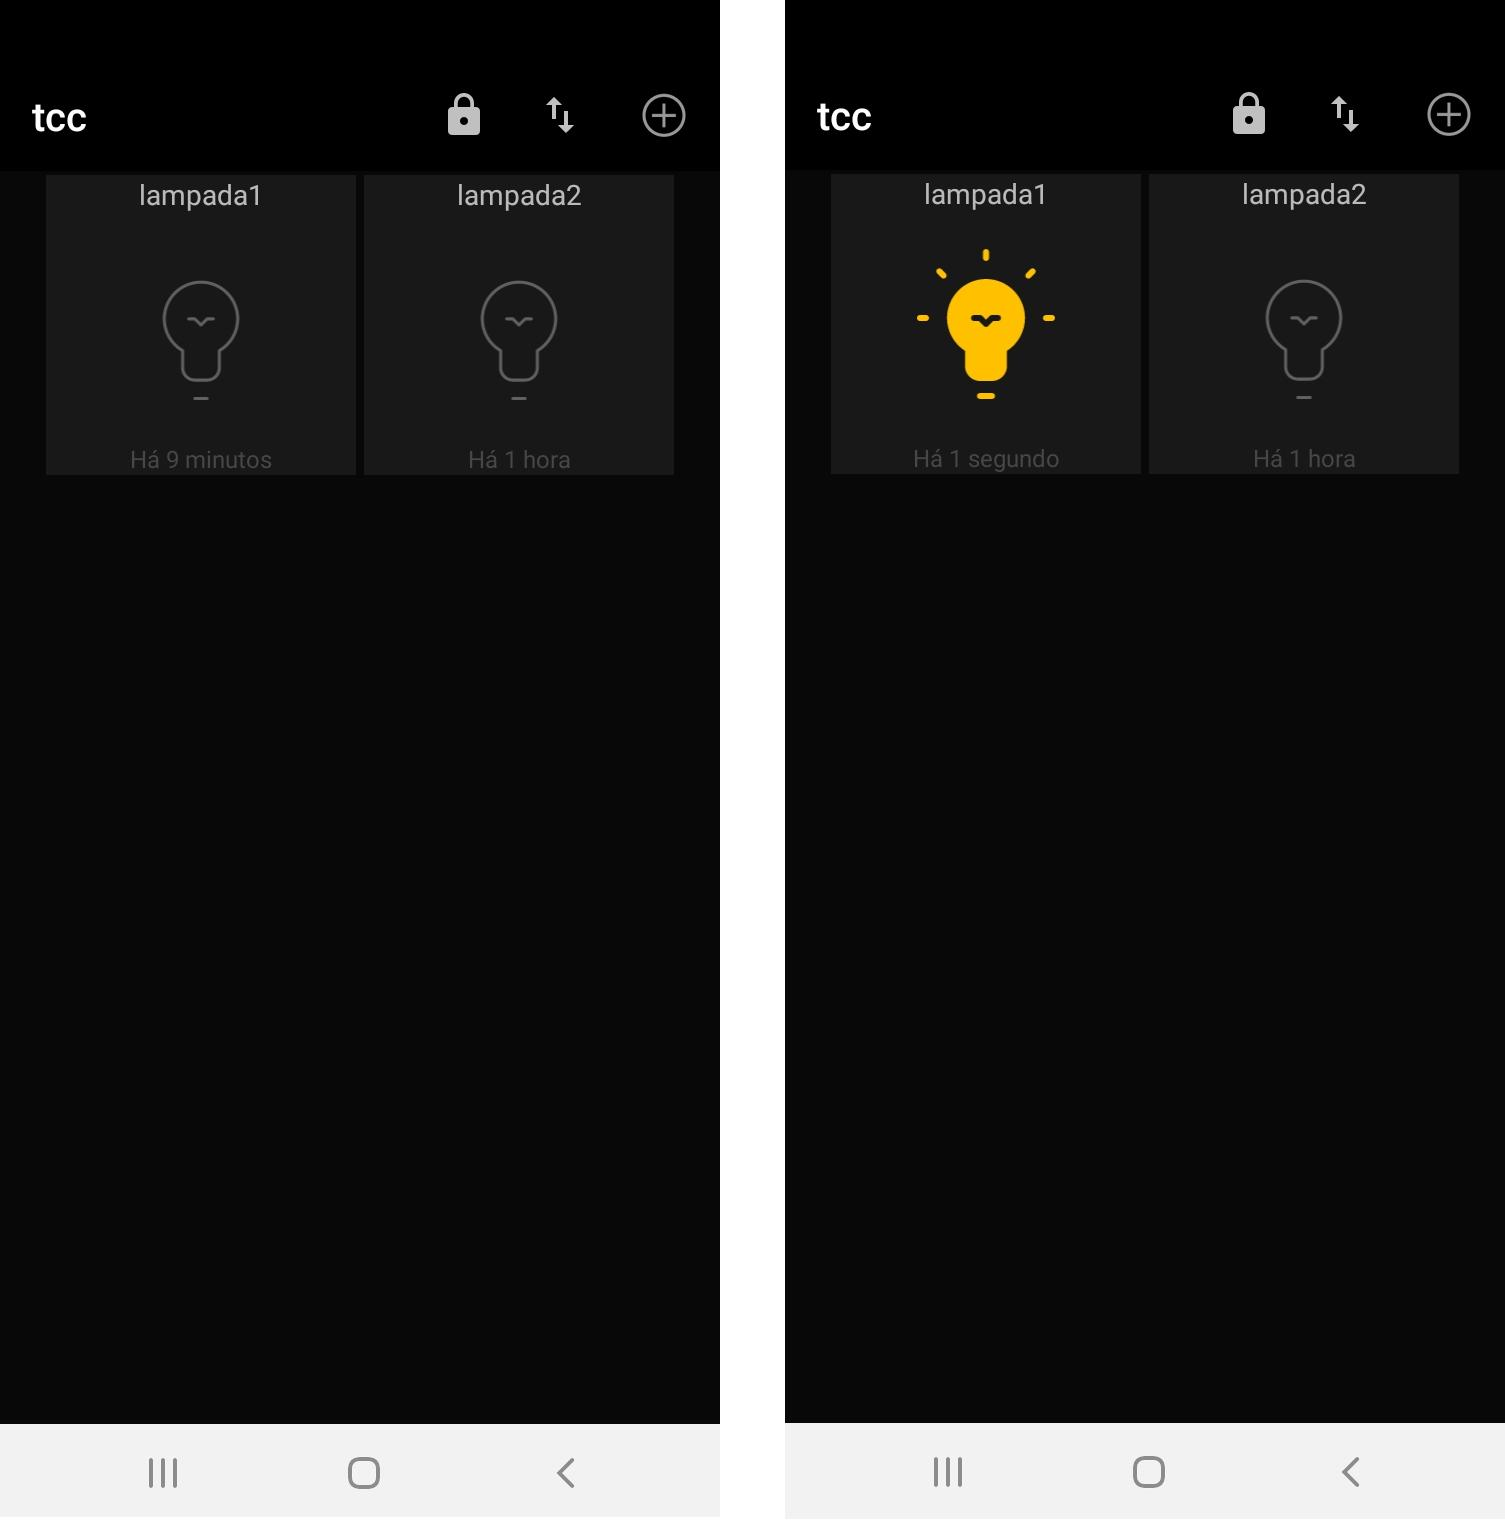
\includegraphics[scale=0.3]{Figuras/app.jpeg}
		\caption{Tela do aplicativo com as lâmpadas desligadas (esquerda) e Tela do aplicativo com uma lâmpada ligada (direita)}
		\label{app}
		\par Fonte: Autor, 2021.
	\end{figure}
	
	

	\chapter{RESULTADOS E ANÁLISES}
	
	Um fato interessante é que para acessar o \textit{Raspberry} através do VNC não foi necessária uma conexão física entre a placa e o \textit{notebook} que funcionou como tela e teclado para este. A placa esteve conectada ao roteador \textit{Wi-Fi} durante todo o funcionamento do projeto, o que era já esperado uma vez que os dados serão recebidos e enviados através do protocolo TCP/IP.
	
	
	As dificuldades encontradas no projeto se resumiram na programação em \textit{Python} e na comunicação do aplicativo MQTT \textit{Dash} com o \textit{Raspberry}. Entretanto, foi obtido êxito na realização das atividades propostas no resumo deste trabalho.
	
	
	
	\chapter{CONCLUSÕES}
	
	\section{Conclusões}
	
	A finalidade deste projeto foi construir uma aplicação de um sistema de automação residencial de baixo custo com capacidade de acionamento de cargas elétricas por meio de uma interface gráfica e da comunicação com um servidor em nuvem. Deste modo, é possível aumentar a segurança, comodidade, o conforto e o grau de acessibilidade a portadores de necessidades especiais.
	
	Uma contribuição direta deste projeto consiste em despertar o interesse acadêmico, notadamente para alunos de graduação, para esta área do conhecimento que possui um conjunto bastante amplo de aplicações, além de um forte apelo social.
	
	Destaca-se a simplicidade e a versatilidade do \textit{software} de gerenciamento, que possui acesso através da Internet e suporte a dispositivos móveis sem fio, como celulares. Esta característica possibilita o monitoramento e controle remoto de todo o sistema.
	
	
	
	\section{Trabalhos Futuros}
	
	 Como melhoria, um segundo código seria elaborado para a criação de uma interface de fácil acesso para enviar e receber informações do dispositivo embarcado. Este segundo código importa a biblioteca \textit{kivy} para criar a interface. É possível ainda com o mesmo código da interface gerar um arquivo ``.apk'' e instalá-lo em um sistema Android.
	 
	 A evolução do projeto para aplicação em uma residência é o objetivo final. Melhorar a qualidade de vida dos usuários será possível inclusive para o caso de mais cargas conectadas e controladas pelo Raspberry - que não foi possível a implementação neste trabalho devido a indisponibilidade de componentes.
	 
	 O monitoramento de ambientes também é foco dos trabalhos futuros. Monitorar quanto tempo as cargas estão ligadas em casa buscando uma redução na conta de energia, emitindo um alerta através de SMS e/ou do próprio aplicativo caso seja atingido um número máximo de horas, definido pelo usuário, da carga ligada.
	



	%% ----------------------------------------------------------
	
	%% ELEMENTOS POS-TEXTUAIS
	
	\postextual
	
    
	%% Referencias. LISTAR EXATAMENTE AS CITADAS NO TRABALHO.
	
	%BIBLIOGRAFIA COM BIBTEX
	%\bibliographystyle{apalike} %PARA USAR BIBTEX DEPOIS
    \bibliographystyle{abntex2-alf}
    \bibliography{Bibliografia}

% Vitor, não vamos colocar seu código no trabalho para evitar plágio.
% É muito comum o plágio de software.


%\begin{apendicesenv}
%	
%\chapter{CÓDIGO PYTHON DA REDE}
%	
%\lstinputlisting{Artigo.py}
%	
%\begin{verbatim}
%#tensorflow==1.15.2
%#keras==2.0.6
%#python==3.6
%
%# ***Imports***
%
%import numpy as np
%import matplotlib.pyplot as plt
%import pandas as pd
%import os
%import random
%import tensorflow as tf
%import keras
%from keras.models import Sequential
%from keras.layers import Dense
%from keras.layers import Dropout
%from keras.layers import LSTM
%from keras.layers import GRU 
%from keras import optimizers
%from keras.callbacks import EarlyStopping
%from keras.callbacks import ModelCheckpoint
%from keras.models import load_model
%from keras import backend as K
%import math
%
%# ***Defines Seed***
%
%def init_seed(seed_value):
%    os.environ['PYTHONHASHSEED'] = str(seed_value)
%
%    random.seed(seed_value)
%    np.random.seed(seed_value)
%    tf.compat.v1.set_random_seed(seed_value)
%
%    session_conf = tf.compat.v1.ConfigProto(intra_op_parallelism_threads=1, 
%    inter_op_parallelism_threads=1)
%    sess = tf.compat.v1.Session(graph=tf.compat.v1.get_default_graph(), 
%    config=session_conf)
%    tf.compat.v1.keras.backend.set_session(sess)
%    
%init_seed(1000)
%
%# ***Loads all the data***
%
%output = pd.read_csv('CMO_certo.csv')
%%input1 = pd.read_csv('Energia_Natural_Afluente_certo.csv')
%input2 = pd.read_csv('Demanda_Maxima_certo.csv')
%input3 = pd.read_csv('Energia_Acumulada_certo.csv')
%input4 = pd.read_csv('Geracao_de_Energia_certo.csv')
%input5 = pd.read_csv('Preço_Gasolina.csv')
%input6 = pd.read_csv('Intercambio_Total.csv')
%
%# ***Transforms the data into arrays and normalizes it***
%
%data_output = output.iloc[:,0].values
%maximo = max(data_output)
%minimo = min(data_output)
%data_output = (data_output - min(data_output)) / (max(data_output) 
%- min(data_output))
%
%data_input1 = input1.iloc[:,0].values
%data_input1 = (data_input1 - min(data_input1)) / (max(data_input1) 
%- min(data_input1))
%
%data_input2 = input2.iloc[:,0].values
%data_input2 = (data_input2 - min(data_input2)) / (max(data_input2) 
%- min(data_input2))
%
%data_input3 = input3.iloc[:,0].values
%data_input3 = (data_input3 - min(data_input3)) / (max(data_input3) 
%- min(data_input3))
%
%data_input4 = input4.iloc[:,0].values
%data_input4 = (data_input4 - min(data_input4)) / (max(data_input4) 
%- min(data_input4))
%
%data_input5 = input5.iloc[:,0].values
%data_input5 = (data_input5 - min(data_input5)) / (max(data_input5) 
%- min(data_input5))
%
%data_input6 = input6.iloc[:,0].values
%data_input6 = (data_input6 - min(data_input6))*2 / (max(data_input6) 
%- min(data_input6)) -1
%
%
%# ***Separates the data into groups of N time steps defined by 
%Tamanho_Temporal*** 
%
%X1 = []
%X2 = []
%X3 = []
%X4 = []
%X5 = []
%X6 = []
%X = []
%Y = []
%
%Tamanho_Temporal = 18
%
%Tamanho_teste = 52
%
%for i in range(Tamanho_Temporal, len(data_output)):
%    X1.append(data_input1[i-Tamanho_Temporal+2:i+1])
%    X2.append(data_input2[i-Tamanho_Temporal+2:i+1])
%    X3.append(data_input3[i-Tamanho_Temporal+2:i+1])
%    X4.append(data_input4[i-Tamanho_Temporal+2:i+1])
%    X5.append(data_input5[i-Tamanho_Temporal+2:i+1])
%    X6.append(data_input6[i-Tamanho_Temporal+2:i+1])
%    Y.append(data_output[i])
%    
%X1 = np.array(X1)
%X2 = np.array(X2)
%X3 = np.array(X3)
%X4 = np.array(X4)
%X5 = np.array(X5)
%X6 = np.array(X6)
%Y = np.array(Y)
%
%# ***Reshapes the data into 3-dimensional arrays with 
%[samples, time steps, features] for feeding into the LSTM***
%
%X1 = np.reshape(X1, (X1.shape[0], Tamanho_Temporal-1,1))
%X2 = np.reshape(X2, (X2.shape[0], Tamanho_Temporal-1,1))
%X3 = np.reshape(X3, (X3.shape[0], Tamanho_Temporal-1,1))
%X4 = np.reshape(X4, (X4.shape[0], Tamanho_Temporal-1,1))
%X5 = np.reshape(X5, (X5.shape[0], Tamanho_Temporal-1,1))
%X6 = np.reshape(X6, (X6.shape[0], Tamanho_Temporal-1,1))
%
%# ***Divides the data set into TRAINING and EVALUATION***
%
%Y_train = Y[0 : len(Y)-Tamanho_teste]
%Y_teste = Y[len(Y)-Tamanho_teste : len(Y)]
%
%X1_train = X1[0 : len(X1)-Tamanho_teste]
%X1_teste = X1[len(X1)-Tamanho_teste : len(X1)]
%
%X2_train = X2[0 : len(X2)-Tamanho_teste]
%X2_teste = X2[len(X2)-Tamanho_teste : len(X2)]
%
%X3_train = X3[0 : len(X3)-Tamanho_teste]
%X3_teste = X3[len(X3)-Tamanho_teste : len(X3)]
%
%X4_train = X4[0 : len(X4)-Tamanho_teste]
%X4_teste = X4[len(X4)-Tamanho_teste : len(X4)]
%
%X5_train = X5[0 : len(X5)-Tamanho_teste]
%X5_teste = X5[len(X5)-Tamanho_teste : len(X5)]
%
%X6_train = X6[0 : len(X6)-Tamanho_teste]
%X6_teste = X6[len(X6)-Tamanho_teste : len(X6)]
%
%
%# ***Puts together all the features into one single 3-dimensional array***
%
%X_train = np.c_[X1_train, X2_train, X3_train, X4_train]
%X_teste = np.c_[X1_teste, X2_teste, X3_teste, X4_teste]
%
%
%# ***Creates the neural network***
%
%model = Sequential()
%
%model.add(LSTM(units = 6, return_sequences = True, input_shape = 
%(Tamanho_Temporal-1,np.shape(X_train)[2])))
%model.add(Dropout(0.15))
%
%model.add(LSTM(units = 8, return_sequences = False, input_shape = 
%(Tamanho_Temporal-1,np.shape(X_train)[2])))
%model.add(Dropout(0.15))
%
%model.add(Dense(1, activation = 'relu'))
%
%
%# ***Defines the loss to be used on the network***
%
%global last
%global last_pred
%
%last = 0
%last_pred = 0
%
%def custom_loss(last1, last_pred1):
%    def loss(y_true, y_pred):
%        verdadeiro = last1 + y_pred - last_pred1
%        global last
%        global last_pred
%        last = y_true
%        last_pred = y_pred
%        return abs(y_true - verdadeiro)
%    return loss
%
%
%# ***Compiles the neural network***
%
%model.compile(optimizer = 'adam', loss = custom_loss(last, last_pred))
%
%# ***Trains the neural network***
%
%checkpoint = ModelCheckpoint
%('Best.h5', save_best_only=True, monitor='val_loss', mode='min')
%history = model.fit(X_train, Y_train, epochs = 360, batch_size = 6, 
%validation_data = [X_teste, Y_teste], callbacks = [checkpoint])
%model.load_weights('Best.h5')
%
%# ***Plots the error history along training epochs for both 
%training and validation sets***
%
%plt.plot(history.history['loss'], label='train')
%plt.plot(history.history['val_loss'], label='evaluation')
%plt.legend()
%plt.grid(True)
%plt.show()
%
%# ***Predicts the outcome of the network for the evaluation data***
%
%predicted = model.predict(X_teste)
%predicted = predicted*(maximo-minimo) + minimo
%Y_teste = Y_teste*(maximo-minimo) + minimo
%
%# ***Plots the predicted X real data for the evaluation set***
%
%plt.plot(Y_teste, color = 'red', label='real')
%plt.plot(predicted, color = 'blue', label='predito')
%plt.legend()
%plt.grid(True)
%plt.show()
%
%# ***Predicts the outcome of the network for the training data***
%
%predicted_train = model.predict(X_train)
%predicted_train = predicted_train*(maximo-minimo) + minimo
%Y_train = Y_train*(maximo-minimo) + minimo
%
%# ***Plots the predicted X real data for the training set***
%
%plt.plot(Y_train, color = 'red', label='real')
%plt.plot(predicted_train, color = 'blue', label='predito')
%plt.legend()
%plt.grid(True)
%plt.show()
%
%# ***Improves the performance of the prediction by setting the real 
%predicted output to be the last real value plus the difference 
%between the last prediction and the current prediction***
%
%arrumado = [Y_teste[0]]
%for k in range(1, np.size(Y_teste)):
%    arrumado.append(Y_teste[k-1] + (predicted[k] - predicted[k-1]))
%
%# ***Creates a comparison for the performance of the prediction. 
%It will be compared to the real values shifted in time by 1***
%
%comparacao = [arrumado[0]]
%for n in range(0, len(Y_teste)-1):
%    comparacao.append(Y_teste[n])
%
%# ***Calculates the mean of the difference between real and 
%predicted values for both the predicted and the comparison sets***
%
%Diferença_absoluta = 0
%Diferença_ponderada = 0
%
%for m in range(0, len(Y_teste)):
%    Diferença_absoluta += abs(Y_teste[m] - arrumado[m])
%    if Y_teste[m] < 50:
%        Diferença_ponderada += abs(Y_teste[m] - arrumado[m]) / 
%        (Y_teste[m] + 50)
%    else:
%        Diferença_ponderada += abs(Y_teste[m] - arrumado[m]) / Y_teste[m]
%        
%Diferença_absoluta /= len(Y_teste)
%Diferença_ponderada /= len(Y_teste)
%
%Diferença_absoluta1 = 0
%Diferença_ponderada1 = 0
%
%for m in range(0, len(Y_teste)):
%    Diferença_absoluta1 += abs(Y_teste[m] - comparacao[m])
%    if Y_teste[m] < 50:
%        Diferença_ponderada1 += abs(Y_teste[m] - comparacao[m]) / 
%        (Y_teste[m] + 50)
%    else:
%        Diferença_ponderada1 += abs(Y_teste[m] - comparacao[m]) / Y_teste[m]
%        
%Diferença_absoluta1 /= len(Y_teste)
%Diferença_ponderada1 /= len(Y_teste)
%
%# ***Plots the predicted and comparison sets along with the real values***
%
%plt.subplot(211)
%plt.plot(Y_teste, color = 'red', label='real')
%plt.plot(arrumado, color = 'blue', label='predito')
%plt.legend()
%plt.grid(True)
%plt.show()
%
%plt.subplot(212)
%plt.plot(Y_teste, color = 'red', label='real')
%plt.plot(comparacao, color = 'blue', label='predito')
%plt.legend()
%plt.grid(True)
%plt.show()
%
%print('Diferença adquirida', Diferença_absoluta)
%print('Diferença básica', Diferença_absoluta1)
%
%# ***Tries to improve performance by training the network on 
%every evaluation data already predicted before predicting the next***
%
%predicted_teste_aos_poucos = []
%
%Y_teste = (Y_teste - minimo) / (maximo - minimo)
%Y_train = (Y_train - minimo) / (maximo - minimo)
%
%new_training_data = X_train
%new_training_label = Y_train
%
%for j in range(0,len(X_teste)):
%    new_data = np.reshape(X_teste[j], (1, np.shape(X_teste)[1],
%    np.shape(X_teste)[2]))
%    predicted_teste_aos_poucos.append(model.predict(new_data))
%    
%    new_output = np.reshape(Y_teste[j], (1))
%    
%    new_training_data = np.r_[new_training_data, new_data]
%    new_training_label = np.r_[new_training_label, new_output]
%    
%    concatenated_training_data = new_training_data[np.shape
%    (new_training_data)[0]-6:np.shape(new_training_data)[0]-1]
%    concatenated_training_label = new_training_label[np.shape
%    (new_training_label)[0]-6:
%    np.shape(new_training_label)[0]-1]
%        
%    if j%5 == 0:    
%        model.train_on_batch(concatenated_training_data, 
%        concatenated_training_label)
%    
%predicted_teste_aos_poucos = np.reshape(predicted_teste_aos_poucos, 
%(len(predicted_teste_aos_poucos)))
%predicted_teste_aos_poucos = predicted_teste_aos_poucos*(maximo-minimo)
%+ minimo
%
%Y_teste= Y_teste*(maximo-minimo) + minimo
%
%# ***Improves the performance of the prediction by setting the 
%real predicted output to be the last real value plus the difference 
%between the last prediction and the current prediction***
%
%arrumado2 = [Y_teste[0]]
%for k in range(1, np.size(Y_teste)):
%    arrumado2.append(Y_teste[k-1] + predicted_teste_aos_poucos[k] 
%    - predicted_teste_aos_poucos[k-1])
%
%# ***Calculates the mean of the difference between 
%real and predicted values***
%
%Diferença_absoluta2 = 0
%Diferença_ponderada2 = 0
%
%for m in range(0, len(Y_teste)):
%    Diferença_absoluta2 += abs(Y_teste[m] - arrumado2[m])
%    if Y_teste[m] < 50:
%        Diferença_ponderada2 += abs(Y_teste[m] - arrumado2[m]) / 
%        (Y_teste[m] + 50)
%    else:
%        Diferença_ponderada2 += abs(Y_teste[m] - arrumado2[m]) / Y_teste[m]
%        
%Diferença_absoluta2 /= len(Y_teste)
%Diferença_ponderada2 /= len(Y_teste)
%
%# ***Plots the predicted and comparison sets along with the real values***
%
%plt.subplot(211)
%plt.plot(Y_teste, color = 'red', label='real')
%plt.plot(arrumado2, color = 'blue', label='predito')
%plt.title('Modelo Proposto')
%plt.legend()
%plt.grid(True)
%plt.show()
%
%plt.subplot(212)
%plt.plot(Y_teste, color = 'red', label='real')
%plt.plot(comparacao, color = 'blue', label='predito')
%plt.title('Modelo Persistente')
%plt.legend()
%plt.grid(True)
%plt.show()
%
%print('Diferença adquirida', Diferença_absoluta2)
%print('Diferença básica', Diferença_absoluta1)
%
%# ***Sees if the strategy to retrain the network on already 
%used eval data has improved performance***
%
%plt.subplot(211)
%plt.plot(Y_teste, color = 'red', label='real')
%plt.plot(predicted, color = 'blue', label='predito')
%plt.legend()
%plt.grid(True)
%plt.show()
%
%plt.subplot(212)
%plt.plot(Y_teste, color = 'red', label='real')
%plt.plot(predicted_teste_aos_poucos, color = 'blue', label='predito')
%plt.legend()
%plt.grid(True)
%plt.show()
%
%# ***Prints Every Result***
%
%print('Diferença adquirida arrumada              ', 
%round(float(Diferença_absoluta),2), 'e' , 
%round(float(Diferença_ponderada*100),2), '%')
%
%print('Diferença adquirida com treino subsequente', 
%round(float(Diferença_absoluta2),2), 'e', 
%round(float(Diferença_ponderada2*100),2), '%')
%
%print('Diferença basica                          ', 
%round(float(Diferença_absoluta1),2), 'e',
%round(float(Diferença_ponderada1*100),2), '%')
%
%
%Y_train = Y_train*(maximo-minimo) + minimo
%
%comparacao2 = [Y_train[0]]
%for n in range(0, len(Y_train)-1):
%    comparacao2.append(Y_train[n])
%
%
%Diferença_absoluta3 = 0
%
%for m in range(0, len(Y_train)):
%    Diferença_absoluta3 += abs(Y_train[m] - comparacao2[m])
%        
%Diferença_absoluta3 /= len(Y_train)
%
%Diferença_absoluta4 = 0
%
%arrumado4 = [Y_train[0]]
%for k in range(1, np.size(Y_train)):
%    arrumado4.append(Y_train[k-1] + 
%    ( predicted_train[k] -  predicted_train[k-1]))
%
%for m in range(0, len(Y_train)):
%    Diferença_absoluta4 += abs(Y_train[m] - arrumado4[m])
%        
%Diferença_absoluta4 /= len(Y_train)
%
%print('Diferença adquirida no treino             ', 
%round(float(Diferença_absoluta4),2))
%
%print('Diferença basica                          ', 
%round(float(Diferença_absoluta3),2))
%	\end{verbatim}
%	
%	\end{apendicesenv}
%    
%    \begin{anexosenv}
%		
%	\chapter{TERMO DE AUTENTICIDADE}
%	
%	%\begin{folhadeaprovacao}
%	\begin{figure}[h]
%		\centering
%		\includegraphics[scale=0.75]{Figuras/Logo.png}
%	\end{figure}
%	\begin{center}
%		\textbf{Termo de declaração de autenticidade de autoria}\\
%		\vfill
%		%		{\chapterfont \bfseries \insereautor}
%		%		
%		%		\vfill
%		%		\begin{center}
%		%			{\chapterfont\bfseries\inseretitulo \inseresubtitulo}
%	\end{center}
%	%		\vfill
%	
%	\noindent Declaro, sob as penas da lei e para os devidos fins, junto à Universidade Federal de Juiz de Fora, que meu Trabalho de Conclusão de Curso do Curso de Graduação em Engenharia Mecânica é original, de minha única e exclusiva autoria. E não se trata de cópia integral ou parcial de textos e trabalhos de autoria de outrem, seja em formato de papel, eletrônico, digital, áudio-visual ou qualquer outro meio.
%	
%	\noindent Declaro ainda ter total conhecimento e compreensão do que é considerado plágio, não apenas a cópia integral do trabalho, mas também de parte dele, inclusive de artigos e/ou parágrafos, sem citação do autor ou de sua fonte. 
%	
%	\noindent Declaro, por fim, ter total conhecimento e compreensão das punições decorrentes da prática de plágio, através das sanções civis previstas na lei do direito autoral\footnote{{\footnotesize LEI N$\mathrm{^\circ}$ 9.610, DE 19 DE FEVEREIRO DE 1998. Altera, atualiza e consolida a legislação sobre direitos autorais e dá outras providências.}}  e criminais previstas no Código Penal\footnote{{\footnotesize Art. 184. Violar direitos de autor e os que lhe são conexos: Pena – detenção, de 3 (três) meses a 1 (um) ano, ou multa.}}, além das cominações administrativas e acadêmicas que poderão resultar em reprovação no Trabalho de Conclusão de Curso. 
%	
%	\vfill
%	
%	\begin{center}
%		Juiz de Fora, Dia de Mês de 2020.
%	\end{center}
%	
%	\vfill
%	
%	\assinatura{Nome completo -- Vítor Giudice Batista de Araujo Porto \\ Matrícula: 201569018B -- CPF: 015408526-01 } 
%	
%	\vspace{30mm}
%	
%	
%\end{anexosenv}
    
	

	%%% ---
\end{document}
